\section{Experimental Evaluation}
\label{sec:experiments}
In this section we present both qualitative and quantitative  performance evaluations of visual MPC on various manipulation tasks assessing the degree of generalization and comparing different prediction models and cost functions and with a hand-crafted baseline.
In Figures \ref{fig:example_traj} and \ref{fig:tile_2} we present a set of qualitative experiments showing that visual MPC trained fully self-supervised is capable of solving a wide range of complex tasks.
Videos for the qualitative examples are at the following webpage\footnote{https://sites.google.com/view/visualforesight/}.
%%SL.11.21: make sure this URL is correct and consistent throughout the paper
In order to perform quantitative comparisons, we define a set of tasks where the robot is required to move object(s) into a goal configuration. For measuring success, we use a distance-based evaluation where a human annotates the positions of the objects after pushing allowing us to compute the remaining distance to the goal.

\subsection{Comparing Video Prediction Architectures}
\label{subsec:sna_experiments}
We first aim to answer the question: Does  visual MPC using the occlusion-aware SNA video prediction model that includes temporal skip connections outperform visual MPC with the dynamic neural advection model (DNA)\cite{foresight} \emph{without} temporal skip-connections?

	%%SL.10.16: do we use the same test procedure in other subsections too? If so, let's have a separate subsection to describe the experiment, and then separate subsections for results, otherwise there will be a lot of duplication. Don't just staple the experiment sections from different papers together...
	%\todo{\autoref{fig:long_distance_task} shows an example task for the pushing experiment.}
	%%SL.10.16: I think these "bare bones" pictures with no distractors are really boring. Can we mostly show interesting tasks with lots of distractors, and contain the simple pushing tasks in one subsection? If we have lots of pictures of the simple tasks, people will conclude that the method only works with one object in the scene.
	%We collected 20 trajectories with 3 novel objects and 1 training object. \autoref{table:res_dna_sna} shows the results for the pushing experiment. The column \textit{distance} refers to the mean distance between the goal pixel and the designated pixel at the final time-step. The column \textit{improvement} indicates how much the designated pixel of the objects was moved closer to their goal (or further away for negative values) compared to the starting location. The true locations of the designated pixels after pushing were annotated by a human labeler.
	
	%The results in \autoref{table:res_dna_sna} show that our proposed planning cost in \autoref{eq:cost}
	%%SL.10.16: wait, what? I thought this section was evaluating models, not costs? Can we separate these out, first evaluate models, then costs, to reflect the organization in the paper?
	%substantially outperforms the planning cost used in prior work~\cite{foresight}. The performance of the SNA model in these experiments is comparable to the DNA model~\cite{foresight} when both use the expected-distance planning cost, since this task does not involve any occlusions.
	%%SL.10.16: Hmm... OK, perhaps if we're going to evaluate costs and models simultaneously like this, we need to organize the sections more clearly. Maybe it would really help in that case to separate out experiment setup (how the methods care compared) from the results (how they stack up). And for each section, ask yourself: what is the question these experiments are trying to answer? It should be obvious from the writing. Right now, I feel like the experiments section looks too much like experiments sections from different papers stapled together. They need to more integrated and focused on achieving the paper's aims: state the research questions, and explain how each experiment subsection answers one or more of those questions



\begin{table}
\centering
{\footnotesize
\begin{tabular}{lcc}
	\toprule
         &  \thead{moved imp. \\ $\pm$ std err. of mean} &   \thead{stationary imp. \\ $\pm$ std err. of mean}  \\
         \midrule
  DNA \cite{foresight} & 0.83 $\pm$0.25 &  -1.1 $\pm$ 0.2\\ 
  SNA & \textbf{10.6 $\pm$ 0.82} & \textbf{-1.5 $\pm$ 0.2} \\
  \bottomrule
\end{tabular}
}
\caption{Results for multi-objective pushing on 8 object/goal configurations with 2 seen and 2 novel objects. Values indicate improvement in distance from starting position, higher is better. Units are pixels in the 64x64 images.} 
\label{table:mult_obj}
\end{table}

To examine whether our skip-connection model (SNA) helps with handling occlusions, we devised a task that requires the robot to push one object, while keeping another object stationary. When the stationary object is in the way, the robot must move the target object around it. This is illustrated on the left side of \autoref{fig:goingaroundocclusion} in the appendix. While pushing the target object, the gripper may occlude the stationary object, and the task can only be performed successfully if the model can make accurate predictions through this occlusion. These tasks are specified by selecting one starting pixel on the target object, a goal pixel location for the target object, and commanding the obstacle to remain stationary by selecting the same pixel on the obstacle for both start and goal. 

We use four different object arrangements with two training objects and two objects that were not seen during training. We find that, in most cases, the SNA model is able to find a valid trajectory, while the DNA model, that is not able to handle occlusion, is mostly unable to find a solution. The results of our quantitative comparisons are shown in \autoref{table:mult_obj}, indicating that temporal skip-connections indeed help with handling occlusion in combined pushing and obstacle avoidance tasks. 
%%SL.10.16: It would help if the experimental conclusion at the end of this section is an answer to  question posed earlier in the experiments. I also think it makes too big of a deal out of the SNA thing -- this is not the SNA paper, we don't need to push on this so hard!

\subsection{Evaluating Registration-Based Cost Functions}
\label{susbsec:reg_cost_exp}
%%SL.11.21: in formal writing, the word after "-" should be capitalized when writing with title case, so this should be Registration-Based
%%SL.10.16: This is very misleading, all of the experiments are closed-loop!

\begin{table}
	{\footnotesize
		\begin{center}
			\begin{tabular}{lcc}
				\toprule
				%				 & \multicolumn{2}{c}{fraction of successful runs} \\
				& Short & Long \\
				\midrule
				Visual MPC $+$ predictor propagation  & 83\% & 20\% \\
				Visual MPC $+$ OpenCV tracking  & 83\%  & 45\% \\
				Visual MPC $+$ registration network & 83\% & \textbf{66\%}  \\
				\bottomrule
			\end{tabular}
		\end{center}
	}
	\caption{\small Success rate for long-distance pushing experiment with 20 different object/goal configurations and short-distance experiment with 15 object/goal configurations. Success is defined as bringing the object closer than 15 pixels to the goal, which corresponds to around $7.5cm$.}
	\label{table:res_long_short}
\end{table}
In this section we ask: How important  is it to update the model's belief of where the target objects currently are? 
We first provide two qualitative examples: In example (1) of Figure \ref{fig:example_traj}
%%SL.11.21: capitalize "figure" (because Figure 1 is the "name" of the figure)
the task is to bring the stuffed animal to a particular location in 3D-space on the other side of the arena. To test the system's reaction to perturbations that could be encountered in open-world settings, during execution a person knocks the object out of the robot's hand. The experiment shows that visual MPC is able to naturally perform a new grasp attempt and bring the object to the goal.
%%SL.11.21: I'm not sure how to interpret this -- where is it shown that visual MPC can perform a new grasp? the figure certainly doesn't show it. Is it shown in the video? if so reference the video

In figure \ref{fig:push_retry}
%%SL.11.21: capitalization
in the appendix, the task is to push the bottle to the point marked with the green dot. In this the system recovers from an initial failure.
%%SL.11.21: I have no idea what this is saying -- there is basically no explanation of what to look for.

The next question we investigate is: How much does this
%%SL.11.21: what does "this" refer to?
matter for short horizon versus long horizon tasks? 
In this experiment, we disable the gripper control, which requires the robot to push objects to the target. We compare two variants of updating the positions of the designated pixel when using a pixel-distance based cost function. The first is a cost function that uses our registration-based method, trained in a fully self-supervised fashion, and the second is with a cost function that uses off-the shelf tracking from OpenCV \cite{babenko2009visual}. Additionally we compare to visual MPC,
%%SL.11.21: isn't it all visual MPC?
which uses the video-prediction model's own prior predictions to update the current position of the designated pixel, rather than tracking the object with registration or tracking.

%SL.10.16: Before talking about videos, explain what this experiment section is actually studying! What is the question? What are you evaluating? Why?

%%SL.10.16: again, not entirely clear what question this is trying to answer

%\begin{figure}
%	\centering
%	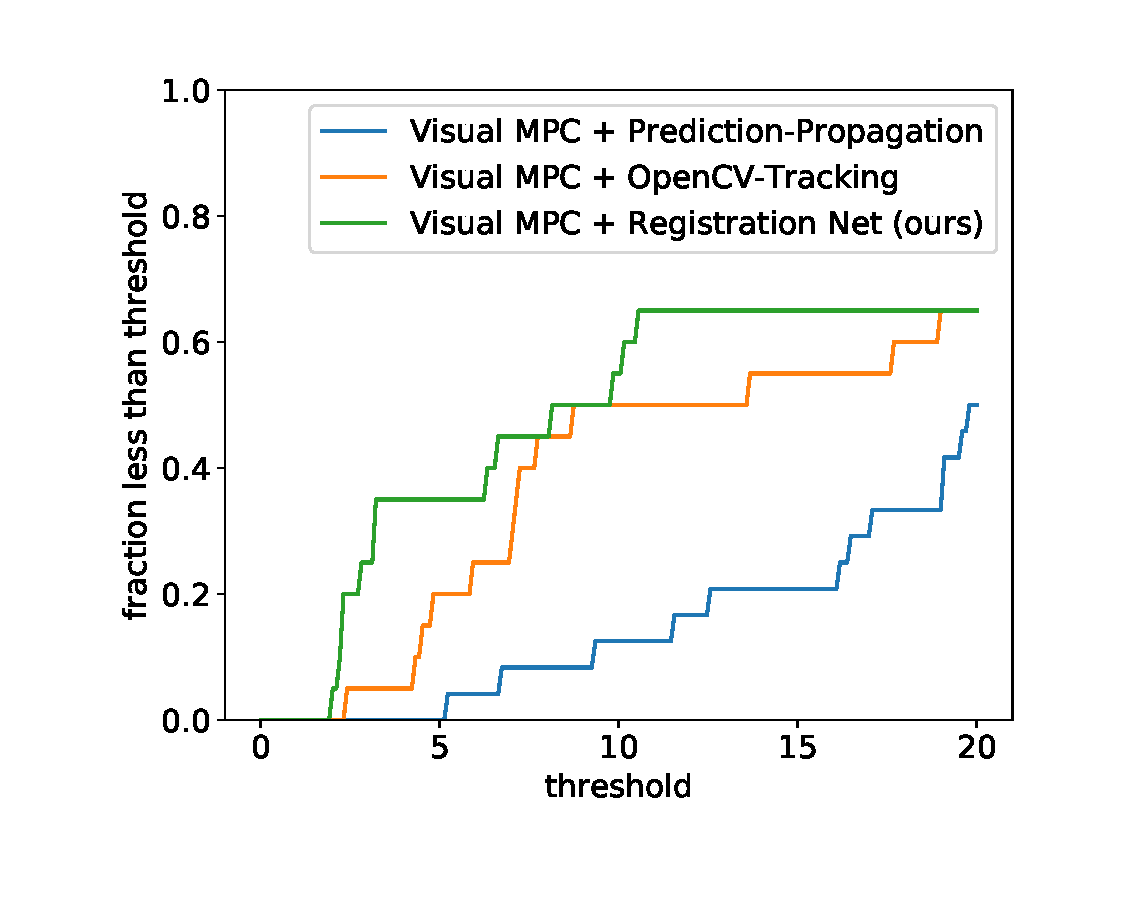
\includegraphics[width=0.8\columnwidth]{images_rfr/pushlong_bench_same_range.pdf}
%	\caption{\small{Results for long pushing tasks with 20 objects not seen during training, showing fraction of runs where final distance is lower than threshold. Our method shows a clear gains over OpenCV tracking and predictor propagation.}}
%	\label{fig:push_bench_long}
%\end{figure}

We evaluate our method on 20 long-distance and 15 short-distance pushing tasks. For long distance tasks the initial distance between the object and its goal position is $30cm$ while for short distance tasks it is $15cm$. Table \ref{table:res_long_short} lists quantitative comparisons showing that on the long distance experiment
visual MPC using the registration-based cost not only outperforms prior work \cite{sna}, but also outperforms the hand-designed, supervised object tracker \cite{babenko2009visual}. By contrast, for the short distance experiment,
all methods perform comparably. Thus, theses results demonstrate the importance of closed loop control for \emph{long-horizon tasks}, while for short-horizon tasks object tracking appears to be irrelevant. 

\subsection{Evaluating Classifier-Based Cost Function}
\label{subsec:eval_classifier}
%%SL.11.21: In formal writing, the word after "-" is capitalized in title case, so this should be "Classifier-Based"

\begin{figure}
	\centering
	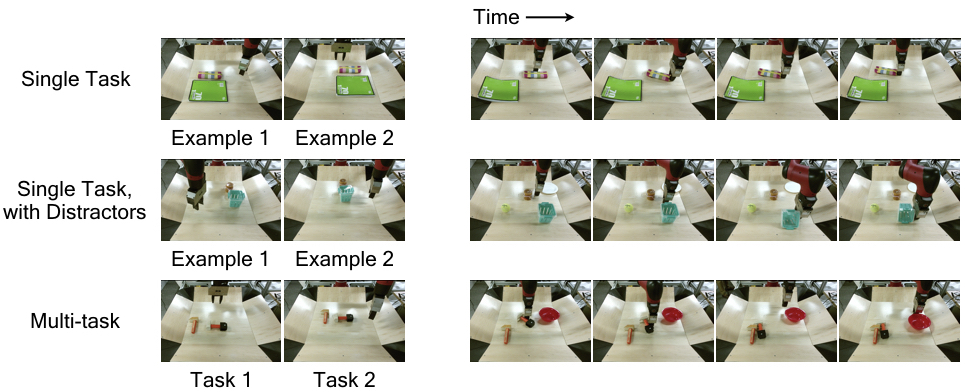
\includegraphics[width=1.0\columnwidth]{images_cls/cls_results_2.jpeg}
	\caption{\small Object arrangement performance of our goal classifier with distractor objects and with two tasks. The left shows a subset of the 5 positive examples that are provided for inferring the goal classifier(s), while the right shows the robot executing the specified task(s) via visual planning.}
	\label{fig:cls_results}
	\vspace{-0.3cm}
\end{figure}

% Here we study the question: How does the success rate of visual MPC using the proposed classifier-based cost function compare to a baseline based on pixel-distance and DSAE in a relative object arrangement task?

The goal of the classifier-based cost function is to provide an easy way to compute an objective for new tasks from a few observations of success for that task, so we compare our approach to alternative and prior methods for doing so under the same assumptions: pixel distance and latent space distance. In the latter, we measure the distance between the current and goal observations in a learned latent space, obtained by training an autoencoder (DSAE) \cite{dsae} on the same data used for our classifier. Since we are considering a different form of task specification incompatible with user-specified pixels, we do not compare the classifier-based cost function to the cost function based on designated pixels.

To collect data for meta-training the classifier, we randomly select a pair of objects from our set of training objects, and position them in many different relative positions, recording the image for each configuration. Each task corresponds to a particular relative positioning of two objects, e.g. the first object to the left of the second, and we construct positive and negative examples for each task by labeling the aforementioned images. We randomly position the arm in each image, as it is not a determiner of task success. A good classifier should ignore the position of the arm. We also include randomly-positioned distractor objects in about a third of the collected images.

We evaluate the classifier-based cost function in three different experimental settings. In the first setting, the goal is to arrange two objects into a specified relative arrangement. The second setting is the same, but with distractor objects present. In the final and most challenging setting, the goal is to achieve two tasks in sequence. We provide positive examples for both tasks, infer the classifier for both, perform MPC for the first task until completion, followed by MPC for the second task. The arrangements of the evaluation tasks were chosen among the eight principal directions (N, NE, E, SE, etc.). To evaluate the ability to generalize to new goals and settings, we use novel, held-out objects for all of the task and distractor objects in our evaluation.

We qualitatively visualize the tasks in Figure~\ref{fig:cls_results}. On the left, we show a subset of the five images provided to illustrate the task(s), and on the left, we show the motions performed by the robot. We see that the robot is able to execute motions which lead to a correct relative positioning of the objects.

We quantitatively evaluate the three cost functions across 20 tasks, including $10$ unique object pairs. A task was considered successfully completed if more than half of the object was correctly positioned relative to the other. The results, shown in Figure~\ref{fig:cls_charts}, indicate that the distance-based metrics struggle to infer the goal of the task, while our approach leads to substantially more successful behavior on average.

%%SL.10.16: what is the conclusion from all this? how do the different methods of specifying costs stack up?

\begin{figure}
    \centering
    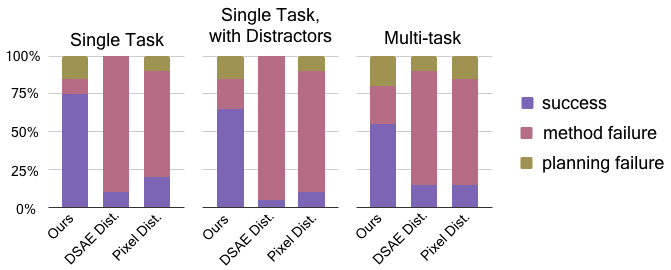
\includegraphics[width=0.48\textwidth]{images_cls/cls_charts_2.jpeg}
    \caption{\small Quantitative performance of visual planning for object rearrangement tasks across different goal specification methods: our meta-learned classifier, DSAE~\cite{dsae}, and pixel error. Where possible, we include break down the cause of failures into errors caused by inaccurate prediction or planning and those caused by an inaccurate goal classifier.}
    \label{fig:cls_charts}
    \vspace{-0.3cm}
\end{figure}


\subsection{Evaluating Multi-Task Performance}
\label{subsec:multi_task_bench}
One of the key motivations for visual MPC is to build a system that can solve a \emph{wide variety} of different tasks, involving completely different objects, physics and, objectives.
%%SL.11.21: I don't think semantics is quite the right term here. Maybe say "objects, physical properties, and smenatic objectives" or something? Still non-ideal though, if you can find a way to avoid "semantic" altogether, that would be better. 
Examples for tasks that can be solved with visual MPC are shown in Figure \ref{fig:example_traj}
%%SL.11.21: The word "figure" should be capitalized, Figure 1 is the "name" of the figure with the number 1, hence it is uppercase. Also, it's a bit awkward to reference a figure on the first page, but I guess there is nothing we can do about it here?
and \ref{fig:tile_2}. Task 1 in Figure~\ref{fig:example_traj} shows a ``placing task" where an object needs to be grasped and placed onto a plate while not displacing the plate. Task 2 is an object rearrangement tasks. The example shown in Task 4 and all examples in Figure \ref{fig:cls_results} show relative object rearrangement tasks. Examples 5 and 6 show the same 3D object positioning tasks from different views. In Task 7, the goal is to move the black object to the goal location while avoiding the obstacle in the middle which is marked with a designated- and goal pixel. 

We also demonstrate that visual MPC -- without modifications to the algorithm -- solves tasks involving deformable objects such as a task where a towel needs to be wrapped around an object (Task 3), or folding a pair of shorts (Task 8). To the best of our knowledge this is the first algorithm for robotic manipulation handling both rigid and deformable objects.

For a full illustration of each of these tasks, we encourage the reader to watch the supplementary video.

The generality of visual MPC mainly stems from two components --- the generality of the visual dynamics model and the generality of the task definition.
We found that the dynamics model often generalizes well to objects outside of the training set, if they have similar properties to the objects it was trained with. For example, Task 8 in Figure \ref{fig:tile_2} shows the model predicting a pair of shorts being folded. The model has never seen shorts during training, towels and shirts were the only clothing items that were part of the training set. In all of these qualitative examples, the predictions are performed by the same model, and the objects are always new objects that were not seen in the training set.
The other source of flexibility for our method is the ability to specify tasks in multiple different ways. Using designated pixels, object positioning tasks can be defined in 3D space, as shown in Task 1 and 2 in Figure~\ref{fig:example_traj} and task 5-6 in Figure~\ref{fig:tile_2}. When adding a goal image, the positioning accuracy can be improved by utilizing the registration scheme discussed in Section \ref{subsec:reg_cost}.
For tasks where we care about \emph{relative} rather than absolute positioning, a meta-learned classifier can be used, as discussed in Section \ref{subsec:class_cost}.

Next, we present a quantitative evaluation to answer the following question: How does visual MPC compare to a hand-engineered baseline on a large number of diverse tasks?

\noindent \textbf{Hand-crafted Baseline} For this comparison, we engineered a simple trajectory generator to perform a grasp at the location of the initial designated pixel, lift the arm, and bring it to the position of the goal pixel. Camera calibration was performed to carry out the necessary conversions between image-space and robot work-space coordinates, which was not required for our visual MPC method. For simplicity, the baseline controller executes in open loop. Therefore, to allow for a fair comparison, visual MPC is also executed open-loop, i.e. no registration or tracking is used.

Altogether we selected 16 tasks, including the qualitative examples presented earlier.
The quantitative comparison is shown in Table \ref{table:cloth_folding}, illustrating that visual MPC substantially outperforms this baseline.
Visual MPC succeeded for most of the tasks. While the baseline succeeded for some of the cloth folding tasks, it failed for almost all of the object relocation tasks. This indicates that an implicit understanding of physics, as captured by our video prediction models, is indeed essentially for performing this diverse range of object relocation and manipulation tasks, and the model must perform non-trivial physical reasoning beyond simply placing and moving the end-effector.


\begin{figure}
	\centering
	\includegraphics[width=1\columnwidth]{images_general/tile_2.png}
	\caption{Visual MPC successfully solves a wide variety of tasks including multi-objective tasks, such as placing an object on a plate (row 5 and 6), object positioning with obstacle avoidance (row 7) and folding shorts (row 8).   
		\label{fig:tile_2}}
\end{figure}

\label{subsec:cloth_folding_data}
\begin{table}
\centering
{\footnotesize
\begin{tabular}{lcc}
	\toprule
         &  \thead{\% of Trials with \\ Final Pixel Distance $< 15$}   \\
         \midrule
  Visual MPC & \textbf{75\%} \\ 
  Calibrated Camera Baseline & 18.75 \% \\
  \bottomrule
\end{tabular}
}
\caption{Results for a multi-task experiment of 10 hard object pushing and grasping tasks, along with 6 cloth folding tasks, evaluating using a single model. Values indicate the percentage of trials that ended with the object pixel closer than 15 pixels to the designated goal. Higher is better.} 
\label{table:cloth_folding}
\end{table}

\subsection{Discussion of Experimental Results}

Generalization to many distinct tasks in visually diverse settings is arguably one of the biggest challenges in reinforcement learning and robotics today. While deep learning has relieved us from much of the problem-specific engineering, most of the works either require extensive amounts of labeled data or focus on the mastery of single tasks while relying on human-provided reward signals. 
From the experiments with visual MPC, especially the qualitative examples and the multi-task experiment, we can conclude that visual MPC \emph{generalizes} to a wide range of tasks it has never seen during training. This is in contrast to many model-free approaches for robotic control which often struggle to perform well on novel tasks. Most of the generalization performance is likely a result of large-scale self-supervised learning, which allows to acquire a rich dynamics model of the environment. 